\setcounter{section}{1}
\section{Ejercicio 2}
El modelo FSP que nos permite generar las trazas dadas como ejemplo en el enunciado se modela como el
siguiente LTS:
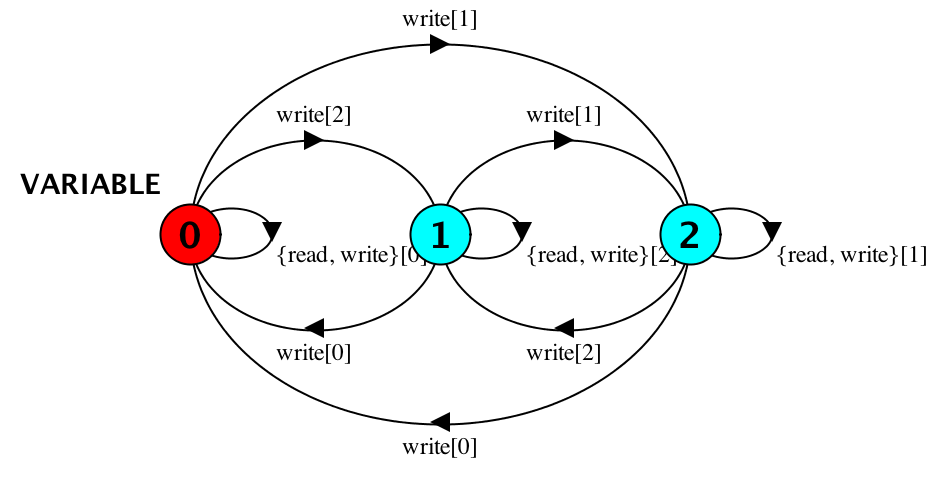
\includegraphics[scale=0.5]{ej2}

El mismo representa una variable de 3 valores posibles (0, 1 o 2) los cuales se van a mantener en el mismo estado mientras se siga leyendo o escribiendo el mismo valor y solo cambiara ́n de estado cuando se escriba otro valor.

\section{Ejercicio 3}
En el siguiente FSP podemos observar el modelo de un sensor que puede tener 10 estados (de 0 a 9).

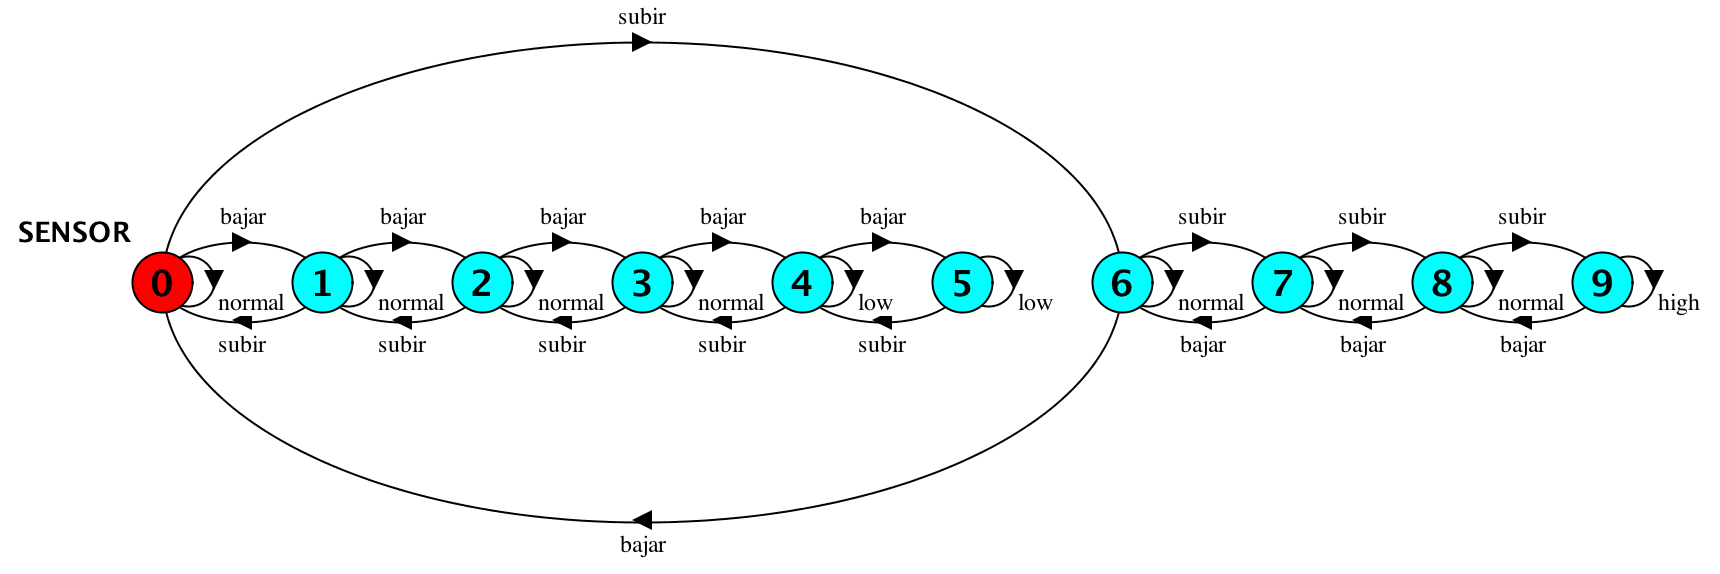
\includegraphics[scale=0.5]{ej3}

El nivel del sensor es inicialmente 5, como vemos puede bajar el nivel 5 veces (hasta llegar a 0) o subir 4 veces (hasta llegar a 9). Cualquier variacion se hace de un paso a la vez, por lo que no pueden haber saltos de estado de más de un nivel por vez.

Por último, los estados de este modelo tienen cada uno una acción apuntando a sí mismos, que representa la emision de una señal correspondiente al nivel del sensor. Para los estados donde el nivel del sensor es 0 o 1, se emite la señal \textit{low}, para el estado donde el nivel es 9, se emite la señal \textit{high}, mientras que para el resto, la señal \textit{normal}.

\section{Ejercicio 4}
Este es el LTS resultante del FSP dado:

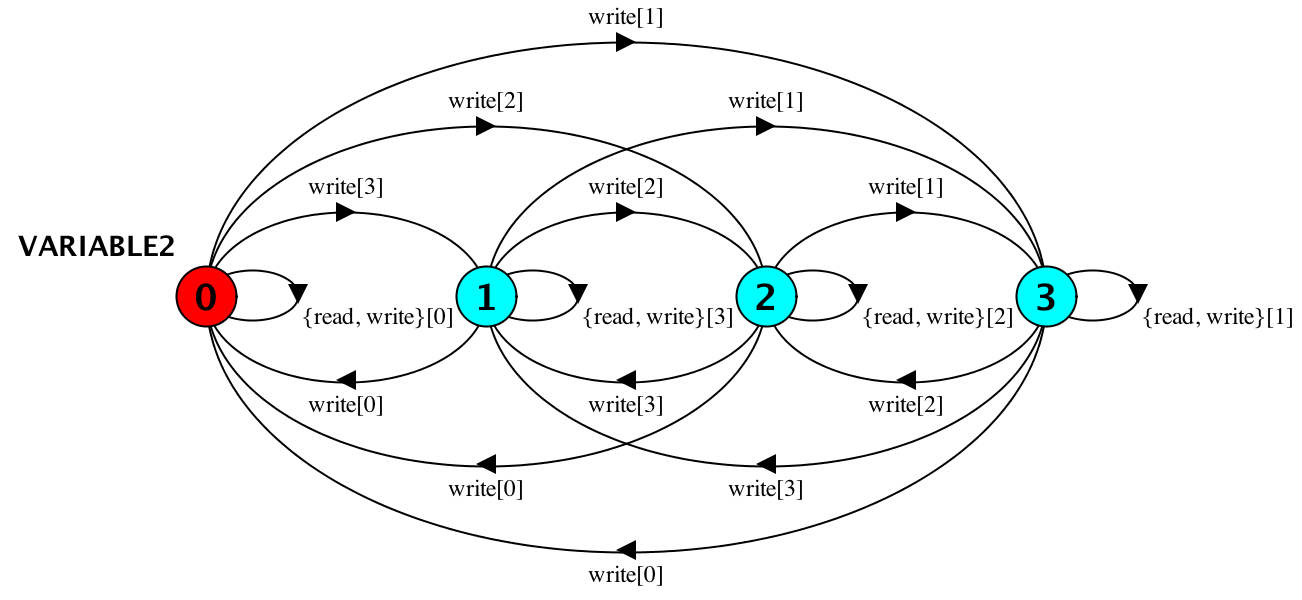
\includegraphics[scale=0.5]{ej4-variable} \\

El LTS de Escritor, cuya única función es enviar la señal de escritura con un valor:

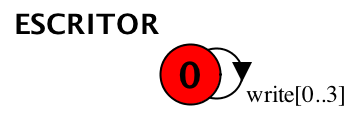
\includegraphics[scale=0.5]{ej4-escritor} \\

El LTS de Lector, que compuesto con variable extiende su funcionalidad ya que además de enviar la señal de lectura, también lo imprime si es distinto de cero:

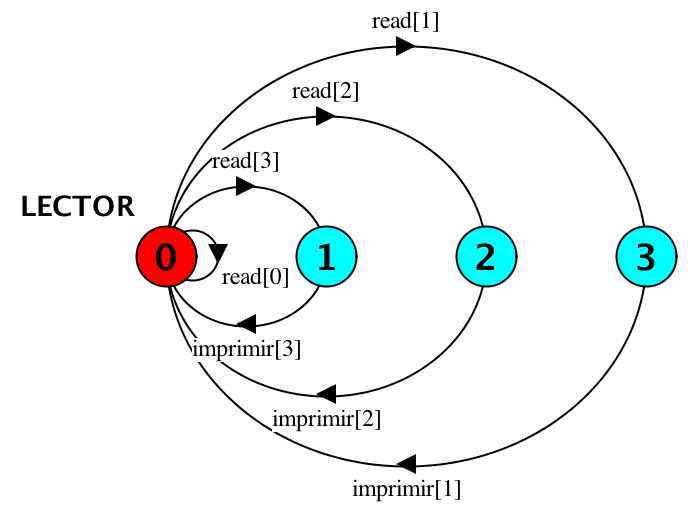
\includegraphics[scale=0.5]{ej4-lector} \\

Finalmente su composición paralela. Aquí podemos observar que se generan una gran cantidad de estados con respecto al LTS de VARIABLE, y esto es debido a la extensión que LECTOR le genera. Siempre puede escribirse distintos valores, pero una vez que ocurra una lectura distinta de cero, se pasa a un estado desde donde no se puede volver a leer hasta imprimir el valor, pero si se puede escribir, por lo que se generan subconjuntos de estados de escritura e impresion (\{2,3,4,5\}, \{7,8,9,10\}, \{12,13,14,15\})

\begin{landscape}
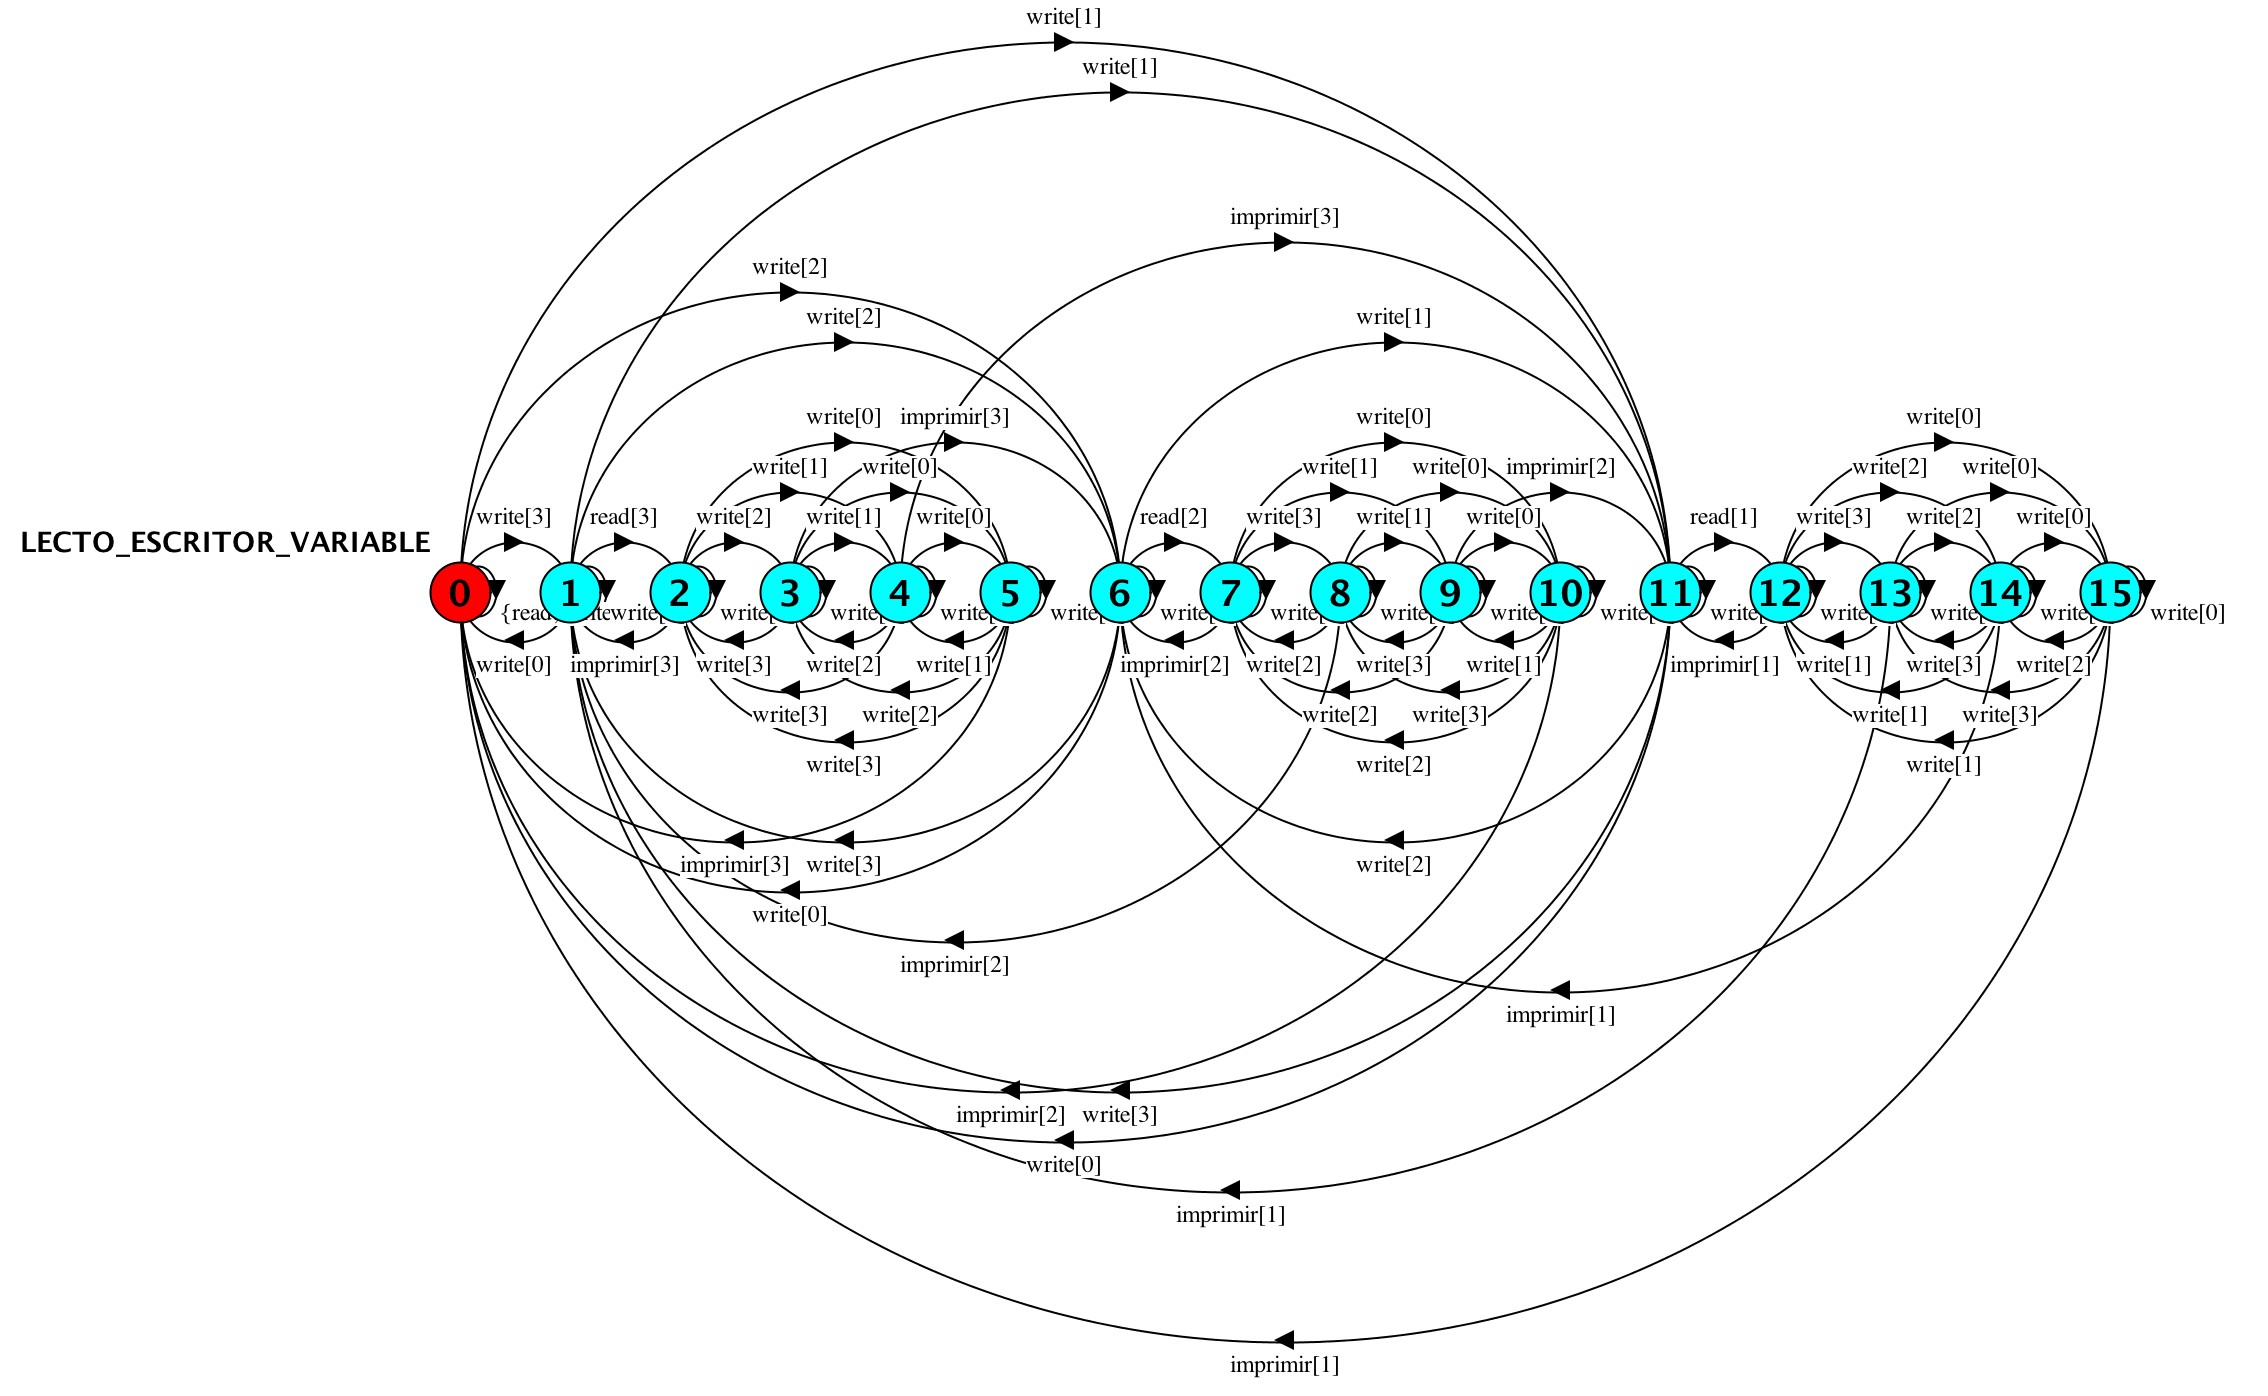
\includegraphics[scale=0.5]{ej4-lecto-escritor-variable} \\
\end{landscape}

\section{Ejercicio 5}
Los LTS de ENTRADA y SALIDA cuya función es simplemente enviar la señal de que alguien entró o salió, respectivamente:

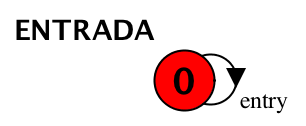
\includegraphics[scale=0.5]{ej5-entrada} 
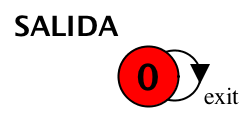
\includegraphics[scale=0.5]{ej5-salida} \\

El LTS del DIRECTOR que se encarga de abrir y cerrar el museo, para luego quedarse esperando a la señal del CONTROLADOR de que el museo ya esta vacío, para poder abrir otra vez:

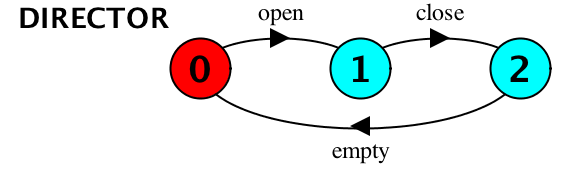
\includegraphics[scale=0.5]{ej5-director} \\

El LTS del CONTROL es el encargado de sincronizar los comportamientos del resto de los procesos. Tiene que saber cuánta gente se encuentra dentro para poder comunicar al DIRECTOR cuándo el museo esta vacío, por lo que cada entrada o salida que reciba de ENTRADA y SALIDA, cambiará de estado al CONTROL. Luego de recibir el cierre por parte del DIRECTOR, evita pasando a un subconjunto de estados que representan que el museo esta cerrado, el cual no permite entradas. Una vez que el museo se vacía, se envía la señal de empty y se queda a la espera de que el DIRECTOR reabra el museo:

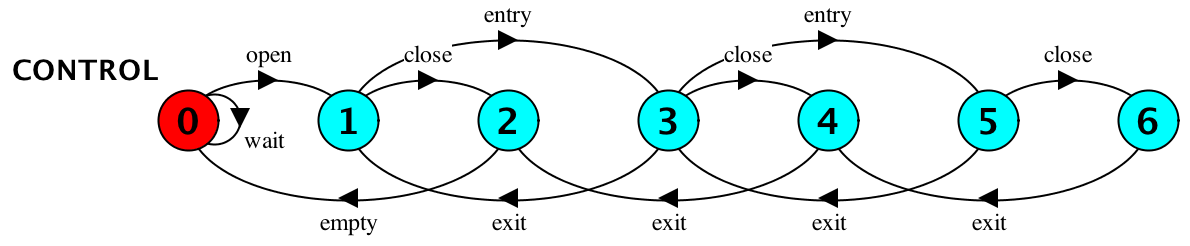
\includegraphics[scale=0.5]{ej5-control} \\

El LTS de la composición paralela es igual al del control ya que en este caso todos los cambios de estado pasan por las decisiones que son reportadas al CONTROL, mientras que el resto de los PROCESOS solo se encarga de reportar:

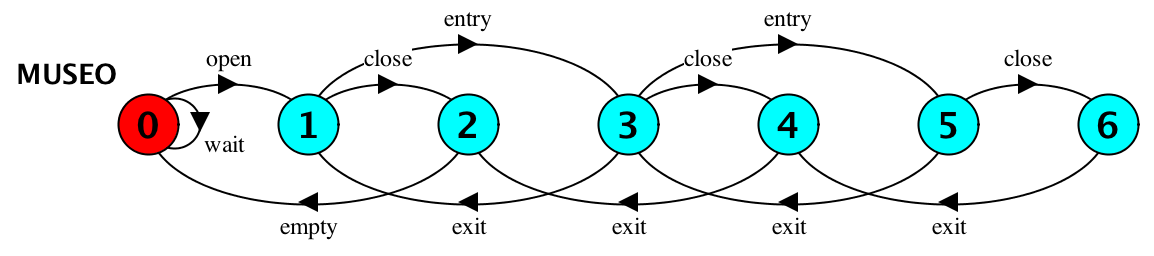
\includegraphics[scale=0.5]{ej5-museo}

\section{Ejercicio 6}
\subsection{}
Este es el LTS de un proceso secuencial equivalente a S:

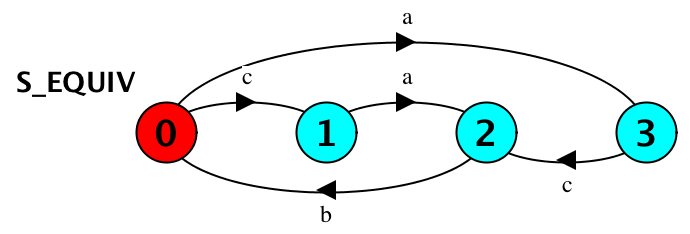
\includegraphics[scale=0.5]{ej6-s-equiv} \\

Aquí es importante notar que es distinto el FSP del LTS anterior: \\

\begin{verbatim}
S_EQUIV = (a -> c -> B | c -> a -> B),
B = (b -> S_EQUIV).
\end{verbatim}

a algo como:

\begin{verbatim}
S_EQUIV = (a -> c -> b -> S_EQUIV | c -> a -> b -> S_EQUIV).
\end{verbatim}

ya que este último generará un LTS que por mas que acepte las mismas trazas, tendrá un estado extra (que como ya vimos con el ejemplo de COIN, no son equivalentes):

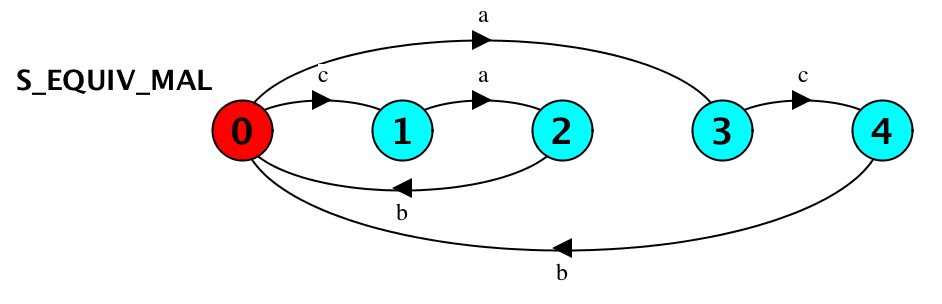
\includegraphics[scale=0.5]{ej6-s-equiv-wrong} \\

Es por esto que utilizamos la etiqueta \textit{B} para demarcar que ambos caminos se crucen en ese estado.

\subsection{}
El proceso \textbf{R} se modela con el siguiente LTS:

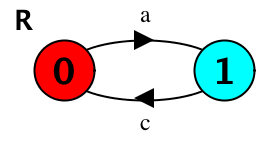
\includegraphics[scale=0.5]{ej6-r} \\

Es importante notar que no sería correcto que \textbf{R} fuera:

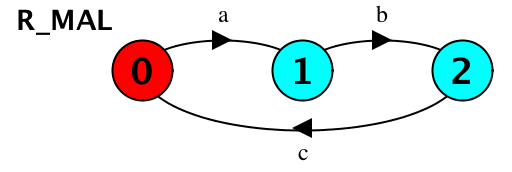
\includegraphics[scale=0.5]{ej6-r-wrong} \\

ya que la restriccíon sería mucho mas fuerte por decir que b tiene que ir después de a y de c. Sin embargo, en este ejercicio, como en \textbf{S} b siempre va después de a y c, la composición con \textbf{S} sería equivalente y es la siguiente:

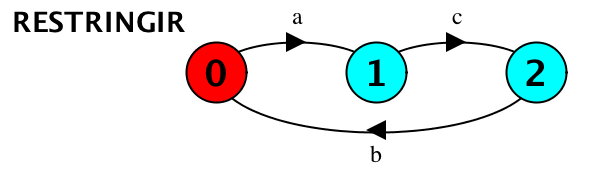
\includegraphics[scale=0.5]{ej6-restringir} \\

\subsection{}
Modelamos \textbf{T} de la siguiente manera:

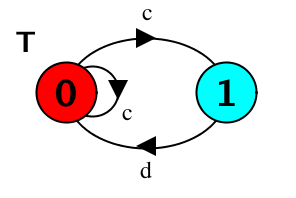
\includegraphics[scale=0.5]{ej6-t} \\

que al componerse con \textbf{S} logra que al observarse \textit{c} o bien ocurra \textit{d} o bien no tener efecto (el auto-loop), lo cual le otorga la opcionalidad:

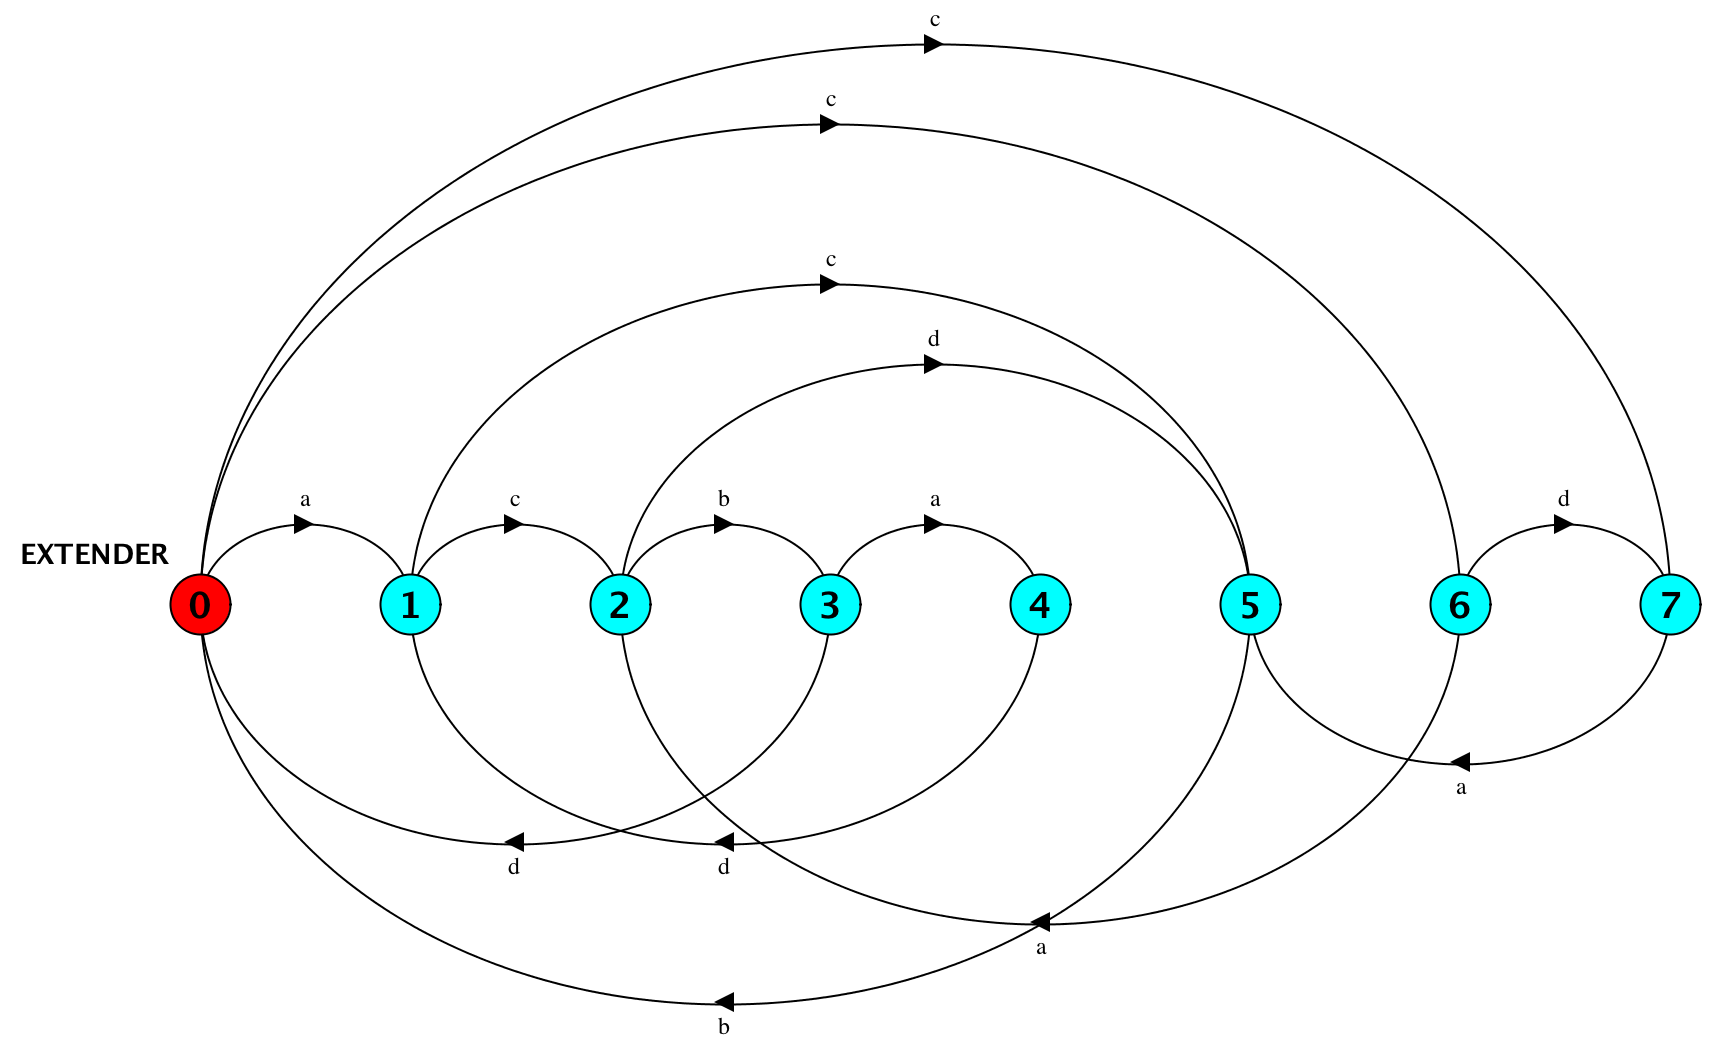
\includegraphics[scale=0.5]{ej6-extender} \\